\newpage
\section{Text-to-Tree transformation}
\genHeader

As we shall see in a moment, libraries and shelves correspond to a folder structure while the contents for a single dictionary are specified in a file.
Figure \ref{fig:moca-4-Tokens} depicts a small sample of the textual syntax used to specify a dictionary. 

\begin{figure}[!htbp]
\begin{center}
 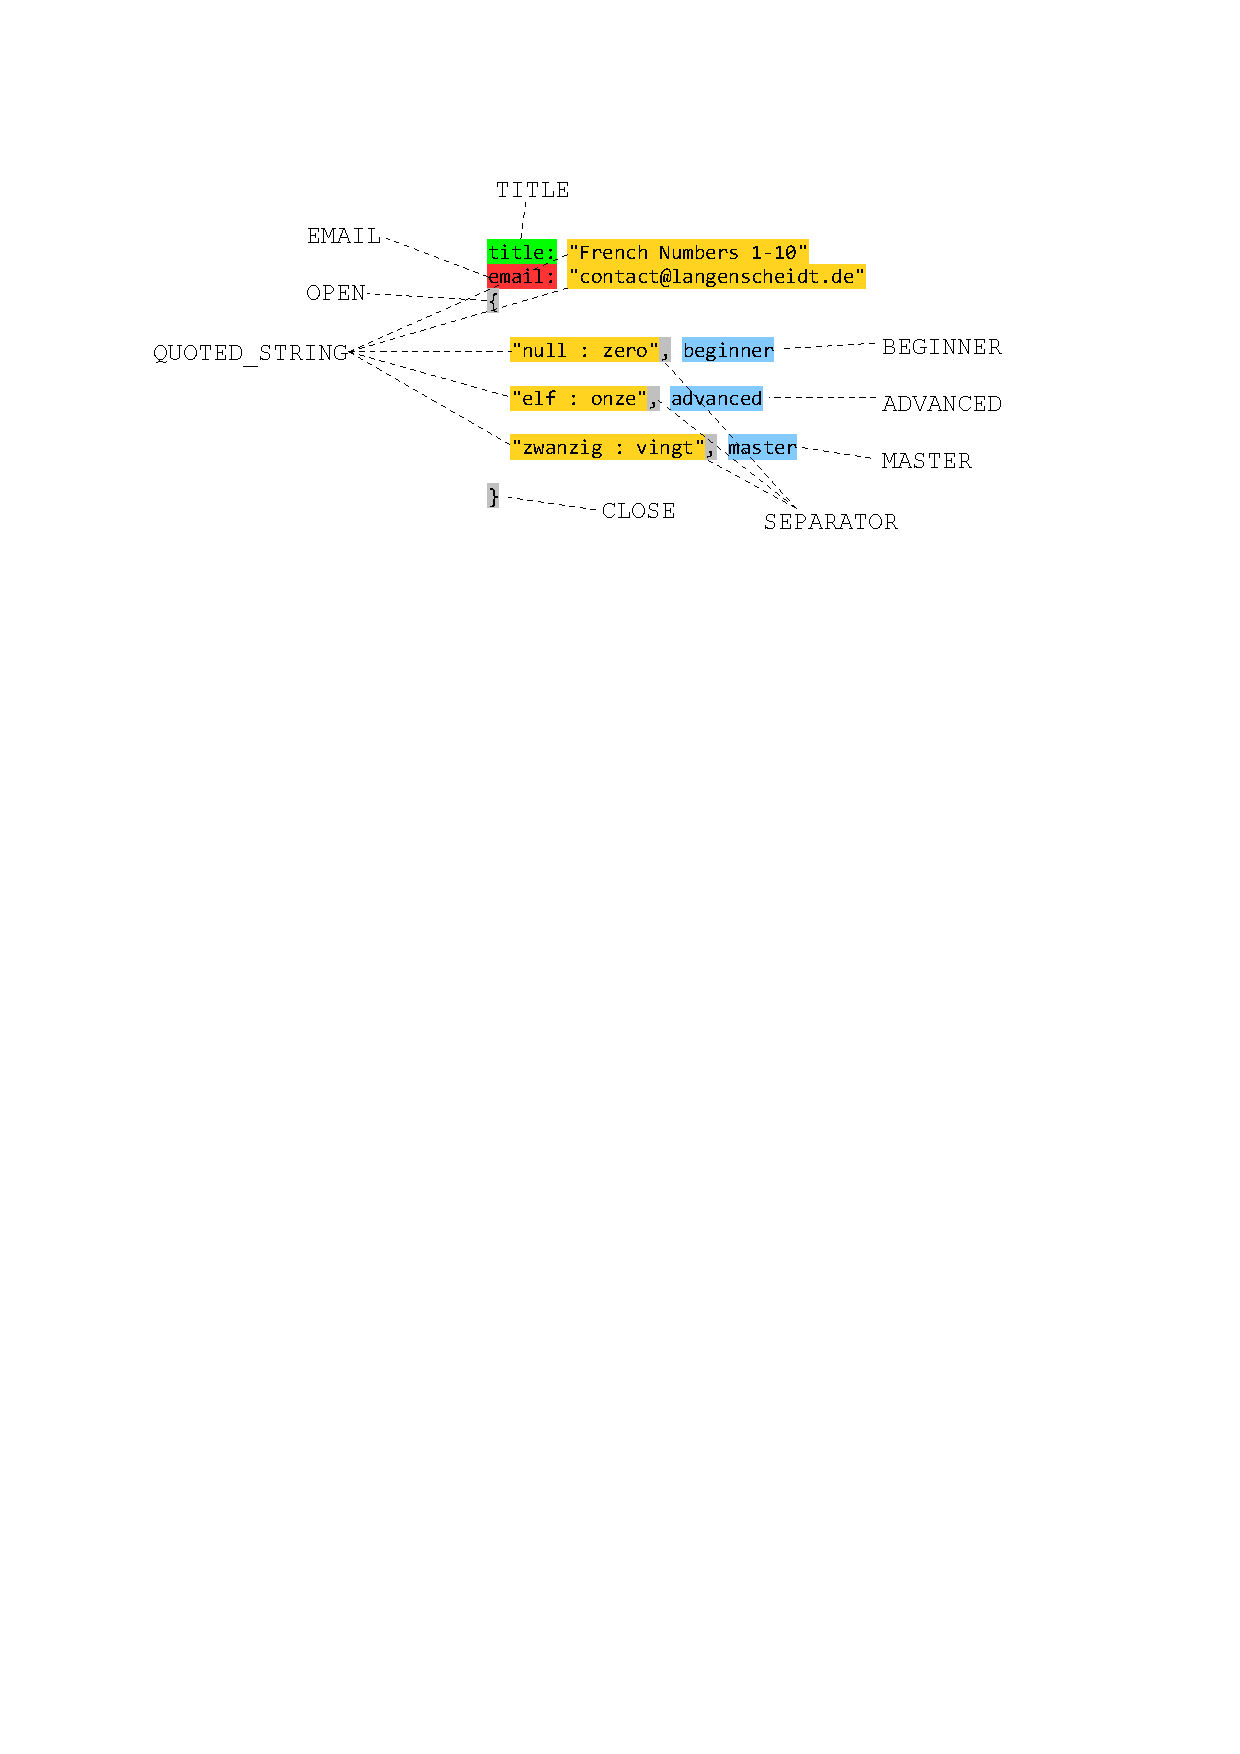
\includegraphics[width=0.7\textwidth]{4-tokens}
  \caption{Identified tokens in a dictionary file \update}
  \label{fig:moca-4-Tokens}
\end{center}
\end{figure}

On the way to an instance model of our dictionary metamodel, the very first step is to create nice \emph{chunks} of characters. This step is called
\emph{lexing} and it simplifies the actual comprehension of the complete text. Interestingly human beings actually comprehend text in a similar manner, one
recognizes whole words without ``seeing'' every individual character. This is the reason why you can siltl raed tihs sneentce alsomt eforftlsesly. A lexer
recognizes these chunks or \emph{tokens} and passes them on as a token stream to the \emph{parser} that does the actual work of recognizing complex
hierarchical and recursive structures.
   
To recognize the tokens as indicated in Fig.~\ref{fig:moca-4-Tokens}, \texttt{ANTLR} can automatically generate a lexer in Java from a compact specification as
depicted in Fig.~\ref{fig:moca-6-lexer}. This is actually a DSL for lexing and is explained in detail in \cite{ANTLR}. If you do not know what EBNF is and have
problems understanding the lexer grammar then make sure you at least go through the documentation on \url{www.antlr.org} or read relevant chapters in
\cite{ANTLR}.

\begin{itemize}
  
\item[$\blacktriangleright$] Edit \texttt{DictionaryLexer.g} so it closely resembles Fig.~\ref{fig:moca-6-lexer}. You'll need to add the \texttt{import
org.moflon.moca.MocaUtil} statment to the header. For the rest of the file, be careful to avoid any typos and mistakes! Save the file to compile it, and ensure
no errors persist.

\end{itemize}
\newpage

\begin{figure}[!htbp]
\begin{center}
  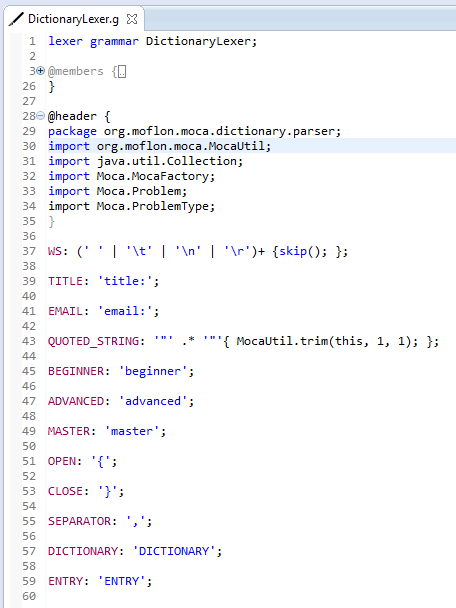
\includegraphics[width=0.7\textwidth]{eclipse_dictionaryLexer}
  \caption{Lexer grammar}
  \label{eclipse:dictionaryLexer}
\end{center}
\end{figure}

Now that we have our lexer built, the next step is to form the stream of tokens from the lexer into a \emph{tree}. In this context, a \emph{tree} is an acyclic,
hierarchical, recursive structure as depicted in Fig.~\ref{eclipse:dictLexer}. Depending on what the tree is to be used for, it can be organized much differently
with extra \emph{structural} nodes such as \texttt{DICTIONARY} or \texttt{ENTRY} that were not present in the textual syntax and are used to give additional
meaning to the tree.

\begin{figure}[htp]
\begin{center}
 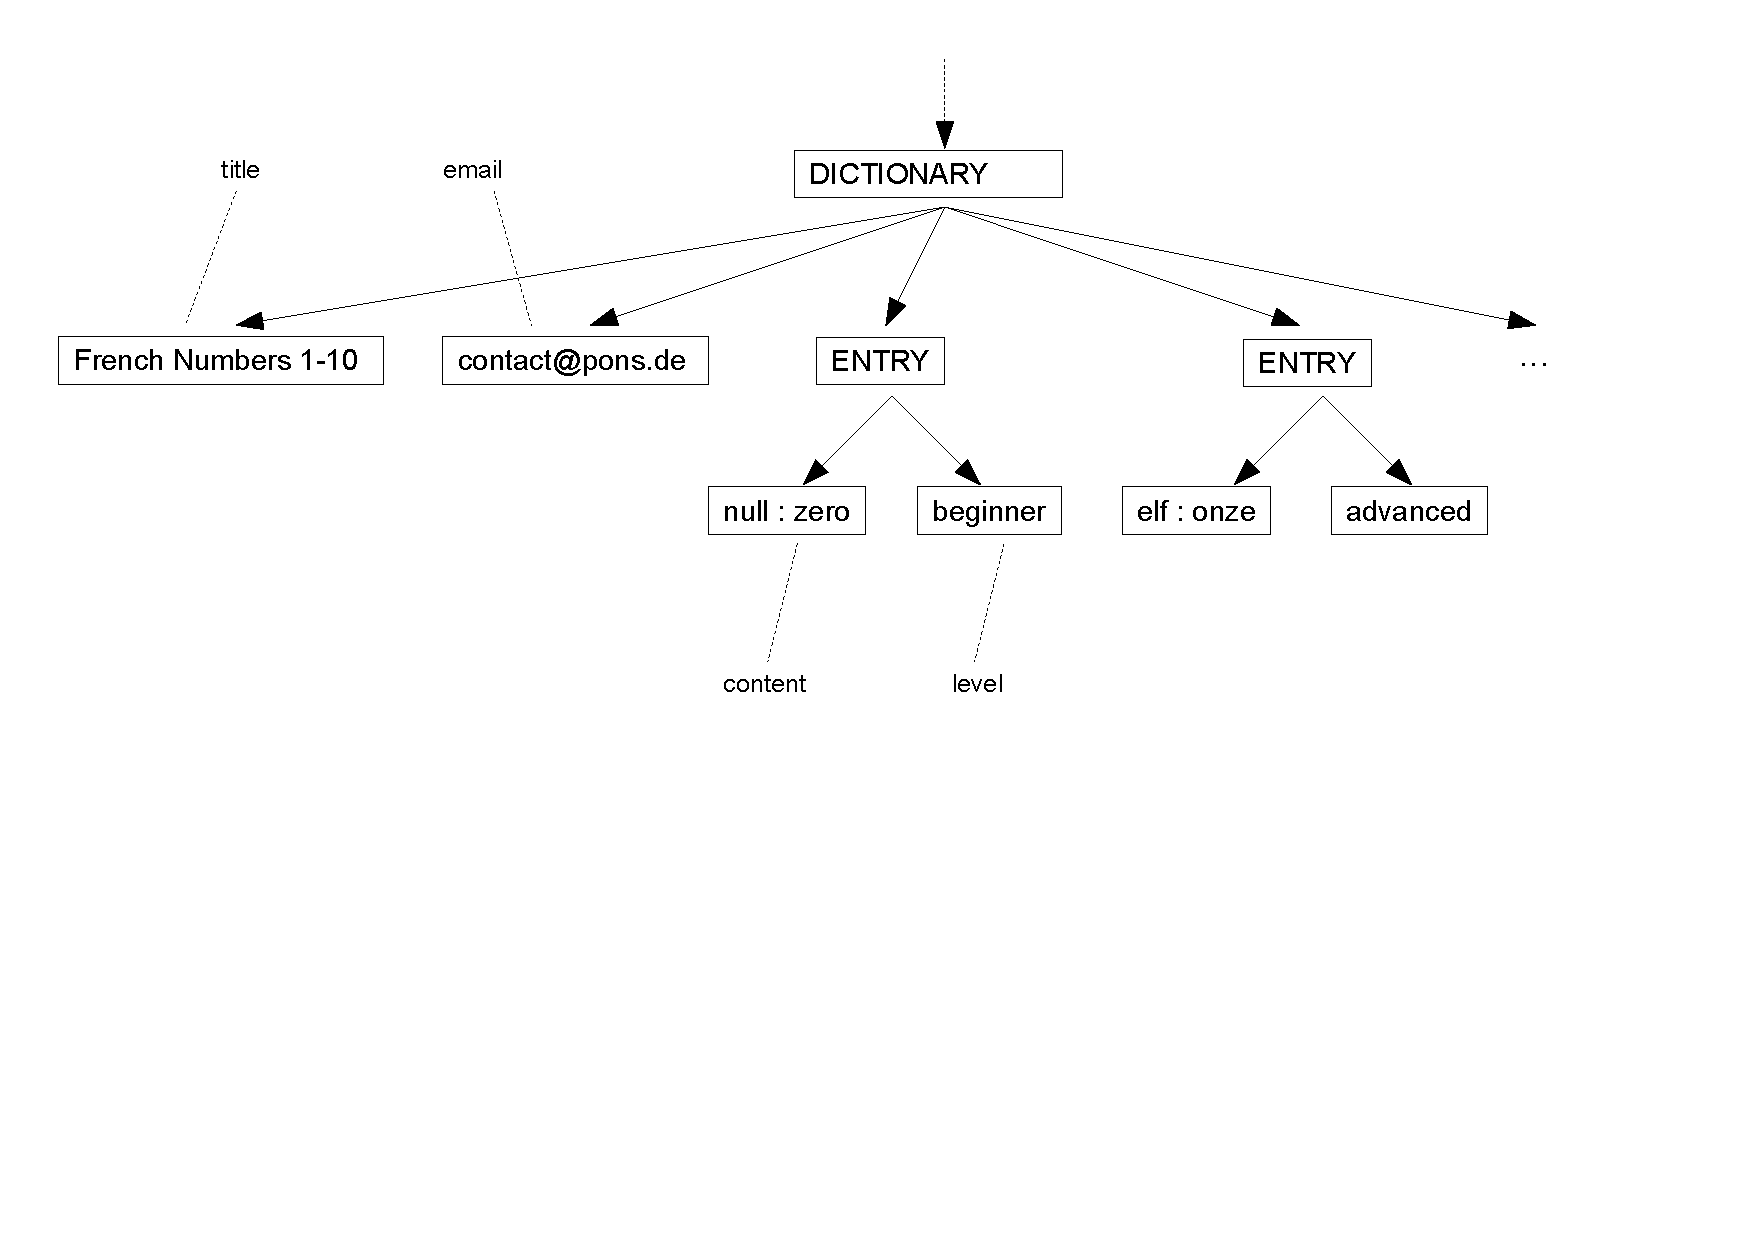
\includegraphics[width=\textwidth]{5-tree}
  \caption{MocaTree structure}
  \label{eclipse:dictLexer}
\end{center}
\end{figure}

\begin{itemize}

\item[$\blacktriangleright$] Open and edit \texttt{DictionaryParser.g} so it closely resembles Fig.~\ref{eclipse:dictParser}. You won't need to make any changes
this time to \texttt{@header}. As with the lexer, avoid typos and mistakes and ensure it compiles before proceeding. Blue are rules, pinkish are values

\end{itemize}

\begin{figure}[!htbp]
\begin{center}
 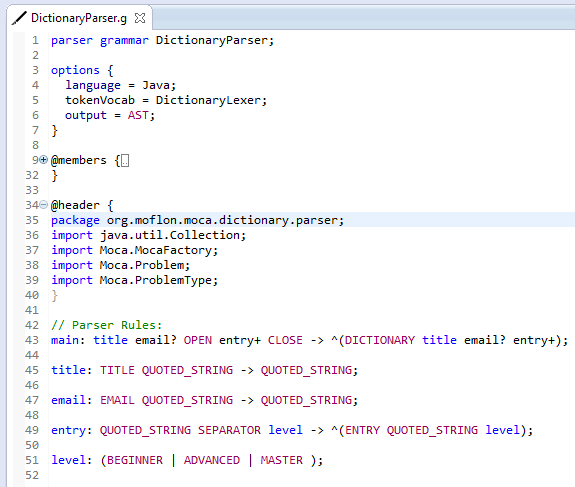
\includegraphics[width=0.9\textwidth]{eclipse_dictionaryParser}
  \caption{Parser grammar}
  \label{eclipse:dictParser}
\end{center}
\end{figure}

As you can see, the parser grammar is quite similar to the lexer grammar, but there are \emph{parser actions} after the \texttt{->} symbol, which build up the
tree. Using this simple tree language, one can (1) abstract from tokens like \texttt{\{} or \texttt{\}}, which are just \emph{syntactical noise}\footnote{In
this context, content that is irrelevant for our model.} and (2) enrich the tree with structural nodes like \texttt{ENTRY}, which add explicit structure to the
tree. Please refer to \cite{ANTLR} and online resources for a detailed explanation of the syntax and semantics of the parser grammar supported by
\texttt{ANTLR}.

{\bf new content }
\begin{enumerate}

\item[$\blacktriangleright$] TGGMAIN: its not the same as it was: explain to users that in INSTANCES/IN source folder.. is the super folder. It will look for
the intial model called tree.xmi. Output/stored files will be in /out. 

\item[$\blacktriangleright$] ** comment out line 46

\item[$\blacktriangleright$]  under //text to tree, the ``Folder folder = MocaMain.getCodeAdapter().parse(new File("instances/in/myLibrary"));'' command will be
the library to be transformed. This may make more sense after working through the example, where you might have several libraries, such as one for languages,
and one for maths.
If you rename your tree.xmi file, this is where you'd have to make the change.

\item[$\blacktriangleright$] To explain, ti takes tree.xmi into the transformer, which in turns creates tree.xmi\_FWD.xmi, an output tree model. This will drive
the backwards transfiormation. (explain the driving process). in other words, this single main method drives the parser, forward transformation, backwards
transformation, and unparser. Streamlined. All you need to start is that inital ``in'' folder with a library directory of some sort. Don't worry about
commenting anything out.


\begin{figure}[htp]
\begin{center}
 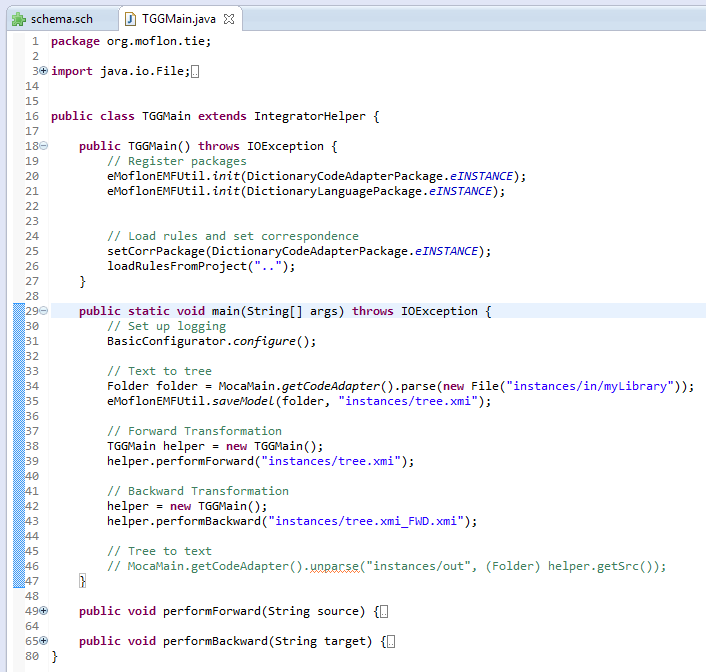
\includegraphics[width=\textwidth]{eclipse_TGGMain}
  \caption{Comment out line 46}
  \label{eclipse:TGGMain} 
\end{center}
\end{figure}

Go ahead and look at what this \texttt{codeAdapter} does. All the code can be adjusted and used, for example, to define which files the parser is
to be used for (per default the adapter registers for \texttt{*.dictionary} files). The main job of the adapter is to hide \texttt{ANTLR} specifics so the
framework remains (parser) technology agnostic. If you decide to use a different parser generator or write the parser by hand you would need to implement a
corresponding adapter from scratch.

On line 27, the input for the framework is set, meaning that all folders in \texttt{./instances/in} are parsed. ((see original!!))
In a nutshell, each folder is taken as a root of a tree and the folder and file structure is reflected as a hierarchy of (children) nodes in the tree.
For each file, the framework searches for a registered parser that is responsible for the particular file, passes the content on to the parser and plugs in the
tree from the parser as a single subtree of the corresponding file node in the overall tree.  

\newpage

The final step is now to prepare some input for the framework ({\bf the in/library folder.}):


\item[$\blacktriangleright$] Navigate to ``DictionaryCodeAdapter/instances/in'' and create the directory structure depicted in Fig.~\ref{eclipse:textDirectory}. You can
create the \texttt{dictionary} files by right-clicking its parent folder, going to ``new/File" and simply appending \texttt{.dictionary} to the end of the name.
Complete each of the four files with the contents from Table~\ref{moca-inputdata}.\footnote{Please do not copy and paste this data as it your .pdf reader may
add some invisible characters to the file that MOSL will not detect}
 
\begin{figure}[htp]
\begin{center}
  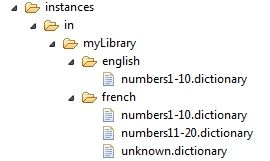
\includegraphics[width=0.5\textwidth]{inputData}
  \caption{Input directory structure.}
  \label{eclipse:textDirectory}
\end{center}
\end{figure}

\end{enumerate}

\newpage

\begin{table}
\begin{tabular}{p{6cm} p{6cm} }
\footnotesize
\textbf{english/numbers1-10.dictionary:}
\begin{verbatim}
title: "numbers1-10"
email: "contact@langenscheidt.de"	
{
  "null : zero", beginner
  "eins : one", beginner
  "zwei : two", beginner
  "drei : three", beginner
  "vier : four", beginner
  "fuenf : five", beginner
  "sechs : six", beginner
  "sieben : seven", beginner
  "acht : eight", beginner
  "neun : nine", beginner
  "zehn : ten", beginner 
}
\end{verbatim} 

\footnotesize
\textbf{french/numbers11-20.dictionary:}
\begin{verbatim}
title: "numbers11-20"
email: "contact@pons.de"	
{
  "elf : onze", advanced
  "zwoelf : douze", advanced
  "dreizehn : treize", advanced
  "vierzehn : quatorze", advanced
  "fuenfzehn : quinze", advanced
  "sechzehn : seize", master
  "siebzehn : dix-sept", master
  "achtzehn : dix-huit", master
  "neunzehn : dix-neuf", master
  "zwanzig : vingt", master
}
\end{verbatim}
&

\footnotesize
\textbf{french/numbers1-10.dictionary:}
\begin{verbatim}   
title: "numbers1-10"
email: "contact@pons.de"	
{
  "null : zero", beginner
  "eins : un/une", beginner
  "zwei : deux", beginner
  "drei : trois", beginner
  "vier : quatre", beginner
  "fuenf : cinq", beginner
  "sechs : six", beginner
  "sieben : sept", beginner
  "acht : huit", beginner
  "neun : neuf", beginner
  "zehn : dix", beginner 
}
\end{verbatim}

\footnotesize
\textbf{french/unknown.dictionary:}
\begin{verbatim}
title: "unknown"
{
	"unbekannt : unknown", beginner
}
\end{verbatim}
  \\
\end{tabular}   
\caption{Input files containing dictionaries.}
\label{moca-inputdata}

\end{table}   

\begin{enumerate}

\item[$\blacktriangleright$] As you can see, you're creating a single library (with the same name as specified in TGGMain) split into two categories, each
containing a number of dictionaries. The syntax of the dictionaries correlate to the lexer/parser in this way..

\item[$\blacktriangleright$] After saving each dictionary, right click on \texttt{TGGMain} and press ``Run As / Java Application.''  you should have an
\texttt{tree.xmi} file. Double-click this to open and inspect the contents FIG

\begin{figure}[!htbp]
\begin{center}
 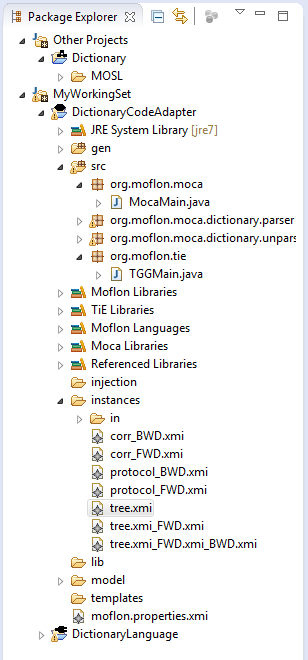
\includegraphics[width=0.4\textwidth]{eclipse_explorerPostGeneration}
  \caption{new tgg file generation result}
  \label{eclipse_postParse}
\end{center}
\end{figure} 

\item[$\blacktriangleright$] \texttt{tree.xmi} file and an \texttt{out} folder (with the same directory structure as \texttt{in}) should be created in the
\texttt{instances} directory after refreshing. EXPLAIN THE NODES AND STUFF HERE.

{\bf mention that we'll do the forwards/backwards transformations in pairs: text to model, model to text, using tree as a middle man?}

\item[$\blacktriangleright$] {\bf this is true}Double-click \texttt{tree.xmi} and compare the contents to Fig.~\ref{eclipse:treeResult}. At this point, you can
reflect on the structure of the tree and note the directory structure, file nodes and the subtrees from the parser. This file is important to understand; The directory
structure is transformed to a corresponding hierarchy of \texttt{Folders} and \texttt{Files}. The actual \emph{textual content} of each file is then transformed
to a subtree using a registered, suitable parser. The resulting subtree from the parser is then plugged into the tree by setting its root as the single child
node of a \texttt{File}.

\end{enumerate}

If everything worked out, well done! You've just completed the first step in the generation:: Text to tree. Now, tree to model to finish the forward
direciton. It follows that it will end with model to tree, then tree to text. You now have a nicely structure tree that we'll be able to use with TGGs and
transform in a few simple steps into an actual instance of our \texttt{Dictionary} metamodel.

\newpage

\vspace*{2cm}

\begin{figure}[!htbp]
\begin{center}
 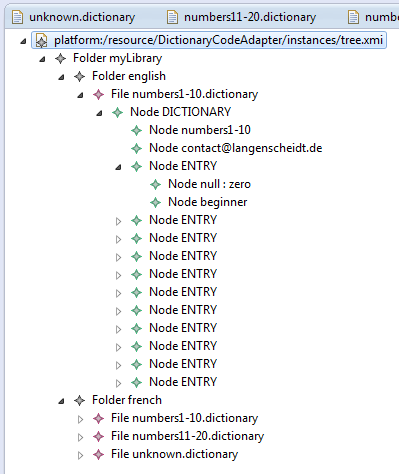
\includegraphics[width=0.6\textwidth]{eclipse_textParsingGeneration}
  \caption{MocaTree created by the framework using our parser}
  \label{eclipse:treeResult}
\end{center}
\end{figure}

